\section{Optimization Setup}
In this section we will set up the requirements and the cost function we want to optimize.

\subsection{Restrictions}
The restrictions are a list of inequetions that our system has to fulfill.
The first restrictions is due to the initial design requirements. The other three are 
somehow arbitrary but will help us to reduce the size of the robot.
\begin{enumerate}
\item We wil place our flywheel in a hole on our robot. We don't want to touch the ground
in any configuration so:
\begin{figure}[ht]
	\centering
	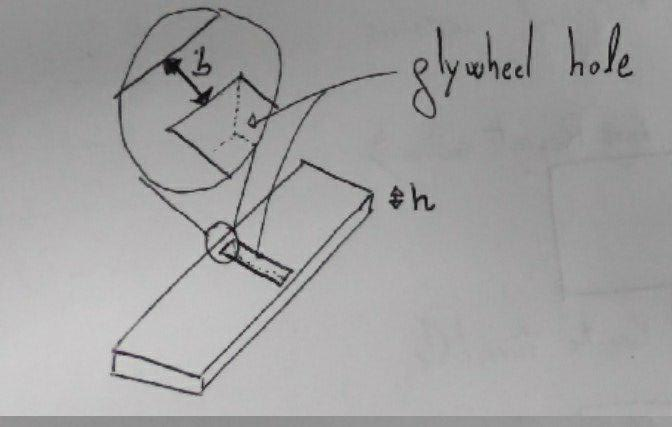
\includegraphics[width=5cm]{img/flywheel_hole.jpg}
	\caption{Flywheel hole diagram}
	\label{fig:Flywheel hole diagram}
\end{figure}
\[r_{wheel}> \sqrt{(r_{flywheel} + b)^2+(\frac{h}{2})^2}\]
\item Being able  to insert the robot in to a wheel of diameter 0.5m so:
\begin{figure}[ht]
	\centering
	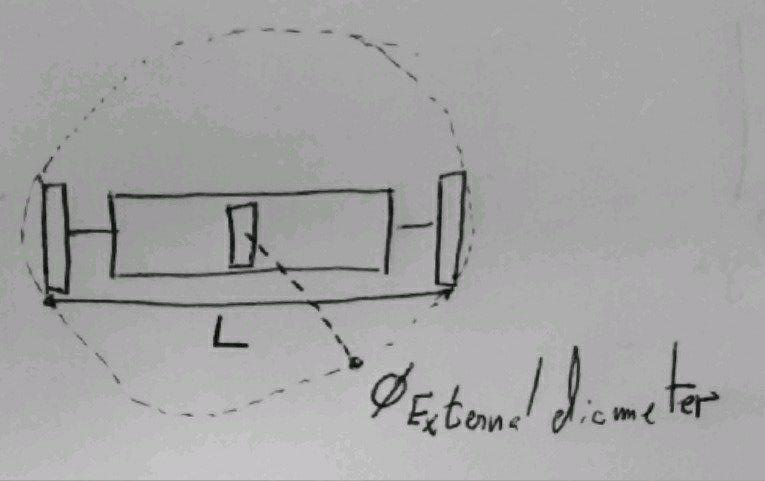
\includegraphics[width=5cm]{img/external_diameter.jpg}
	\caption{External diameter diagram}
	\label{fig:External diameter diagram}
\end{figure}
\[0.25 m > \sqrt{r_{wheel}^2 + L^2/4}\]
\item We can place all electronic the devices:
\[L > 0.3m + w \]
\item Maximum weight of the robot: 5kg
\end{enumerate}

\subsection{Requirements}
We would like our robot to reach some mechanical specifications. This ones are related to mechanical equations
that we will develop in the next section. They refer to the max speed, acceleration and inclination the robot may achieve
while controlling it's inclination. We have divided our specifications in two blocks
according to the two mechanisms.

\textbf{Flywheel mode}
\begin{enumerate}
	\item $\dot{y}_{max}$ (equation \ref{Maximum speed flywheel}) $> 0.1m/s$
	\item $\ddot{y}_{max}$ (equation \ref{maximum acceleration flywheel}) $> 1m/s^2$
	\item $sin(\alpha_{max})$ (equation \ref{Maximum angle using flywheel system}) $>0.2$
\end{enumerate}

\textbf{Pendulum mode}
\begin{enumerate}
	\item $\dot{y}_{max}$ (equation \ref{maximum speed pendulum}) $>1m/s$
	\item $\ddot{y}_{max}$ (equation \ref{maximum acceleration pendulum}) $>0.1m/s^2$
	\item $sin(\alpha_{max})$ (equation \ref{Maximum angle using pendulum system}) $> 0.02$
\end{enumerate}
	


\subsection{Cost function}
In addition to fulfilling the previous inequetions we will
minimize a cost function.

We will maximize the maximum sinus in the pendulum mode 
(equation \ref{Maximum angle using pendulum system}) because
it give the robot the capacity to deliver force in a permanent state.

And we will also maximize the square of the max speed the robot can achieve
in flywheel mode (equation \ref{Maximum speed flywheel}) because it is
proportional to the energy the robot can deliver using the flywheel at a certain moment.

\begin{equation}
	cost(r_{flywheel},r_{wheel},w,N) = - sin(\alpha_{max})_{pendulum} -\dot{y}^2_{max-flywheel}
	\label{eq: cost}
\end{equation}
In the next section we will find out what are the values 
of this equations with the construction parameters. 
For reference this terms are equal to:
\begin{equation*}
	m_{cylinder} = \rho * w * \pi * (\frac{r_{flywheel}}{3})^2
\end{equation*}
\begin{equation*}
	sin(\alpha_{max})_{pendulum} = \frac{m_{cylinder} \cdot  (r_{max} - r_{min})}{m_{total} \cdot r_{wheel}} = \frac{m_{cylinder} \cdot  (\frac{r_{flywheel}}{3})}{(m_{rest} + N \cdot m_{cylinder})\cdot r_{wheel}} 	
\end{equation*}
\begin{equation*}
	\dot{y}_{max} = r_{wheel} \cdot  R \cdot  \dot{\theta}_{max} =r_{wheel} \cdot  \frac{ N \cdot  m_{cylinder} \cdot  (\frac{2\cdot r_{flywheel}}{3})^2}
    {r_{wheel}^2\cdot (m_{rest} + N \cdot m_{cylinder}) +  2\cdot I_{wheel}} \cdot  \dot{\theta}_{max}
\end{equation*}
